\section{Emotionen in der Psychologie}
Historisch gesehen kann man drei  \"{}Zeitalter\"{} von Emotionsforschung der Psychologie klassifizieren \cite{stearns_reconstructing_2009}. Das \"{}Goldene Zeitalter\"{}, welches sich 1855 bis 1899 erstreckt und maßgebliche Emotionstheorien von Darwin und James hervorbrachte. Das \"{}Finstere Mittelalter\"{} (1900-1959), bei welchen aufgrund des aufkommenden Behaviorismus, bei welcher das Verhalten im Forschungsmittelpunkt der Psychologie rückte, Emotionen weitestgehend vernachlässigt wurden. Und die \"{}Renaissance\"{} (ab 1960), in welcher die Rolle von Emotionen komplett neu definiert wurde \cite{anselm_winfried_muller_emotionen_2013}.

Die erste Arbeit im Goldenen Zeitalter über Emotionen. die geschichtlich relevant scheint kommt von Herbert Spencer (1855). Er bezeichnet Erinnerungen, Vernunft und Gefühle als verschiedenen Seiten eines gleichen Psychischen Phänomens. Für ihn tauchen Gefühle, Erinnerungen und Vernunft immer gleichzeitig auf, sie haben also denselben Grund. Er argumentiert auch, dass Kognition, wobei die einfachste Form davon Wahrnehmung wäre, und Emotion, wobei die einfachste Form ein Sinneseindruck wäre, nicht ohne einander auftreten würde. Sinneseindrücke bezeichnet er als primäre unteilbare Zustände des Bewußtseins, während Wahrnehmung sekundäre teilbare Zustände sind die aus Veränderungen primärerer Zustände bestehen. Die einfachen Sinneseindrücke, welche die niedrigste Form von Gefühlen sind können höhere Gefühle hervorrufen indem sie kombiniert werden. So generiert eine Gruppe von Sinneseindrücken und ihre Beziehung zueinander, bzw. auch die Beziehung von verschiedenen Gruppen zueinander eine solche höhere Form eines Gefühls. Als Konsequenz erscheint folgende Feststellung, dass Emotionen nur dann erscheinen, wenn Kognition oder Bewußtsein involviert ist. Bei vollständig automatischen Reaktionen so keine Emotionen möglich.
Dabei impliziert Emotion Kognition, weil eine Emotion auch immer eine Repräsentation oder die Repräsentation eines Objektes oder eines Verhaltens involviert und diese Wahrnehmung von diesen Objekten oder Verhalten immer auch Kognition beinhaltet. Kognition impliziert Emotion, indem bestimmte materielle Wahrnehmungen die einen kognitiven Prozess involvieren auch Sinneseindrücke involvieren, die zu einer Annahme oder Ablehnung der Repräsentation dieser Wahrnehmung führt. Allerdings kann eine solche Emotion die damit Verbunden ist stark oder schwach sein in ihrer Quantität und Intensität.  
Die Stärke eines Gefühls kann durch zwei verschiedene Dinge bestimmt werden: zum einen durch das Ergebnis einer intensiven Anregung ein paar wenigen Nervenzellen und zum anderen durch eine unterschwellige Anregung vieler Nervenzellen. Eine solche Aggregation von psychischen Zuständen können durch ihr auftreten außerdem strukturelle Veränderungen im Nervensystem auslösen. Dabei nimmt er Bezug auf die Plastizität des Gehirns, wobei beim Auftreten von gleichzeitigen Impressionen oder Ereignissen Verbindungen zwischen den Neuronen geschaffen werden, die das Gehirn bzw. die Nervenzellen langfristig ändern. 
Die Power einer Emotion ist dabei proportional zu der Nummer von elementaren Zuständen die im Bewußtsein zu diesem Zeitpunkt vereint werden. In seinem Aufsatz über die Emotionen beschreibt Spencer Angst und Wut, welche von körperlichen Ausdrücken begleitet wird, mit folgender Beschreibung: "Angst, wenn stark, drückt sich in Schreien, in Bemühungen zu verstecken oder zu entkommen, in Herzklopfen und Zittern; Und das sind nur die Manifestationen, die eine wirkliche Erfahrung des Bösen befürchten würden. Die zerstörerischen Leidenschaften sind in einer allgemeinen Spannung des Muskelsystems, im Knirschen der Zähne und des Vorsprungs der Klauen, in erwünschten Augen und Nasenlöchern, in Knurren gezeigt; Und das sind schwächere Formen der Handlungen, die das Töten der Beute begleiten."
Gendron und Barrett verorten in Spencers Theorie den Ursprung aller drei bisherigen psychologischen Emotionstheorien. Die Dimensionale oder auch Psychologische Konstruktions-Theorie, weil Emotionen und Kognition aufgrund desselben Ereignisses auftreten und, weil Emotionen immer eine mentale Repräsentation aus Erfahrungen in der Vergangenheit involvieren. Aufgrund der Beschreibung, dass Emotionen in bestimmten Arealen im Gehirn lokalisiert sind und dass er bestimmte emotionale Klassen beschreibt und diesen spezifische Körperreaktionen zuschreibt, kann man laut Gendron und Barrett seine Theorie auch der Basisemotionstheorie zuschreiben. Und aufgrund der Beschreibung von Emotionen als aufkommende Verhalten zu den  Appraisaltheorien. Allerdings wird aus der Beschreibung und und deren Eingrenzung klar, dass einzelne Aspekte der Theorie aus der Gesamtbeschreibung herausgenommen wird und die passenden Textpassagen den unterschiedlichen Theorien zugeordnet wird. Der ganze komplexen Prozess, den Spencer vor allem auf neurologischer Grundlage beschreibt, wird keine dieser Theorien gerecht.\\

Eine weitere Arbeit des \"{}Goldene Zeitalter\"{} entstand in der Emotionstheorie nach Darwin, welcher die Grundlage für die Basis-Emotionstheorien legte die ihren bekanntesten Vertreter in Paul Ekman gefunden hat. Darwin \cite{darwin_et_al} beschreibt Emotionen als ausgedrückte Zustände des Geistes, welche in ganzer Welt auffällig gleich sind (S. 17). Die Wichtigkeit des expressiven Ausdruck von Emotionen im Gesicht, welche eine Gemütsfassung beschreibt zusammen mit einer Erklärung unter welchen Umständen die erscheinen, würden viel Wert haben (S. 16)). Wie auch die Kognitivisten geht Darwin davon aus, dass körperliche emotionale Reaktionen durch emotionalen geistigen Zustände ausgelöst wird.\\
Darwin beschreibt in seinem Buch "The expression of the emotion in man and animals" Emotionen als bewußte mentale Zustände von Personen oder höheren Lebewesen. Gemäß der von ihm entwickelten Evolutionstheorie geht er davon aus, das bestimmte emotionale Reaktionsverhalten bzw. emotionale Ausdrücke vererbt sind und einen stammesgeschichtlichen Hintergrund haben. Dabei entstehen nach Darwin Emotionen  durch Einschätzungen und Bewertungen von Objekten, Situationen oder Ereignissen. Er beschreibt dabei Emotionen wie Furcht, Wut, Traurigkeit und Überraschung. Überraschung tritt dann auf wenn etwas unerwartetes oder unbekanntes eintritt. Eine solche Emotion geht laut Darwin mit einem Emotionsausdruck einher. Dieser umfasst alle körperlichen Reaktionen, wie Mimik, Gestik, Körperhaltung, Stimmveränderungen und physiologische Veränderungen. Er bezieht sich dabei sogar auf die Veränderung der Herzrate, aufgrund einer Emotionalen Erregung, wie sie Claude Bernard gefunden hat. Er beschreibt 3 Prinzipien auf denen solche Emoionsausdrücke erfolgen.
\begin{enumerate}
\item Das Prinzip der zweckassoziierten Gewohnheiten
\item Das Prinzip der Antithese
\item Prinzip der direkten Tätigkeit des Nervensystems
\end{enumerate}
Das Prinzip der zweckassoziierten Gewohnheiten tritt auf wenn ein bestimmte komplexes, willkürliches Verhalten durch bestimme Gemütszustände ausgelöst wird um damit einen bestimmten Zweck zu erreichen. Zum Beispiel bei visuellen Reizen, dass öffnen der Augen um Sinneseindrücke wahrzunehmen. Diese Ausführungen werden dann unter Umständen zu Gewohnheiten, die wiederum durch evolutionäre Prozesse vererbt werden. Diese Ausdrücke können jedoch durch den Wille unterdrückt und in seinem Erscheinen verändert werden. Das Prinzip der Antithese tritt ein, wenn bestimmte Zustände des Geistes zu gewissen gewohnheitsmäßigen Handlungen führen, die von Nutzen sind, wie unter unserem ersten Prinzip. Wenn nun ein unmittelbar entgegengesetzter Geisteszustand hervorgerufen wird, so herrscht eine starke und unwillkürliche Tendenz zur Aufführung von Bewegungen einer direkt entgegengesetzten Natur, obwohl diese nutzlos sind; Und solche Bewegungen sind in manchen Fällen sehr ausdrucksvoll. Das dritte Prinzip tritt ein, wenn das Sensorium stark angeregt ist, und die Nervenkraft im Übermaß erregt wird und diese Erregungen in gewisse Richtungen übertragen werden, je nach der Verbindung der Nervenzellen und dabei teils zur Gewohnheit werden können. Außerdem kann die Versorgung der Nervenkraft auch unterbrochen werden. Dabei entstehen ebenfalls Effekte, die wir im Ausdruck erkennen.
Für Darwin hat der Ausdruck von Emotionen mehre Funktionen, zum einen eine biologische, das heißt der Ausdruck wurde vererbt. Eine organismische Funktion, das heißt der Ausdruck diente dazu um bestimmte Dinge wahrzunehmen oder den Körper auf bestimmte Dinge vorzubereiten. Und eine kommunikative, dass heißt sie wurden eingesetzt um Artgenossen über den eigenen Zustand, die eigenen Bedürfnisse und Wünsche zu informieren.\\
William James kritisierte diesen Ansatz. Er meinte: "Wir zittern nicht weil wir Angst haben, sondern wir erleben Angst weil wir zittern."
Das heißt er dreht die komplette kausale Kette von Darwin um. Für ihn entstehen Emotionen, weil der Körper auf eine Situation oder Reiz reagiert. Dem emotionsauslösenden Reiz folgt die erste Objekterfassung, aus dieser folgt die körperliche Veränderung, welche dann wahrgenommen wird und dann die empfundene Emotion entsteht. Die empfundene Emotion ist dabei der subjektive Aspekt eine Emotion. 
Er trifft dabei drei Annahmen, die für das Empfinden einer Emotion notwendig sind:
\begin{enumerate}
\item die Wahrnehmung eines Reizes löst eine reflexartige physiologische (viszerale und motorische) Reaktion aus
\item zwischen der Reizwahrnehmung und der körperlichen Reaktion ist kein Bewertungsprozess zwischen geschaltet
\item die körperlichen Veränderungen sind emotionsspezfisch und wahrnehmbar
\item das Empfinden der Veränderungen ist die Emotion
\end{enumerate}
Da unabhängig von James zur gleichen Zeit Carl Lange eine ähnlich Theorie publizierte nennt man die sich daraus gründende Theorie James-Lange-Theorie.\\
Kritik kam zugleich von Cannon der in seiner Schrift 1927 explizit die James-Lange-Theorie angreift. Cannon begründet seine Kritik an empirischen Studien mit Katzen (Cannon, 1992). Darin zeigt er das eine Unterbrechung zwischen Zentralen Nervensystem und Organen zu keinen Totalausfall der Emotionen führte. Desweiteren können dieselben körperlichen Veränderungen, die zu Emotionen führen auch unter anderen nicht emotionalen Ereignissen auftreten, wie zum Beispiel bei Fieber. Vor allem aber sind die körperlichen Antworten auf einen Reiz diffus,und die Reaktionen des zentralen Nervensystems langsam. Desweiteren zeigte Marañon 
(1924) in einer Studie, bei der Probanden Adrenalin gespritzt wurde, dass die dabei gefühlte Emotion nicht in allen Fällen als echten Emotionen wahrgenommen wurden.Die meisten Probanden (70 \%) berichteten starken Emotionen, die sie aber als kalt und unbestimmt wahrnahmen.  Andere Probanden (30 \%) berichteten von meist negativen Gefühlen. Daraus schlussfolgerten die Wissenschaftler dieser Zeit, dass eine körperliche Reaktion nicht ausreicht um eine Emotion zu erzeugen sondern, dass eine Bewertung dieser Reaktion erfolgen muss.\\
Mit Wundt (1905) wurde ein weiterer Grundstein für eine andere Emotionstheorie gelegt, der dimensionalen Emotionstheorie oder auch später die psychologische Konstruktionstheorie genannt (Gendron \& Barrett). Wundt verfolgt einen Sprach- und erlebniszentrierten Ansatz.
Dabei definierte er verschiedene Gefühlszustände, welche sich aus drei Partialgefühlen zusammensetzen sollen. Jedes dieses Partialgefühl ist bipolar, und umfasst Lust/ Unlust, Erregung/ Beruhigung und Spannung/Lösung. Ein Affekt ist bei ihm ein Gefühlszustand mit einem bestimmten dynamischen Verlauf innerhalb dieser Dimensionen (zum Beispiel von Spannung zu Unlust zu Lösung zu Lust).\\
1996 konnte Schmidt-Atzert die Dimensionen Lust/ Unlust und Erregung/ Beruhigung mittels moderner physiologischer Studien über Skalierungsverfahren und Datenreduktion nachweisen. Die Dimension Spannung/ Lösung bzw. die damit verbundene Erwartungshaltung konnte nicht nachgewiesen werden. Allerdings scheint das Konzept der bipolaren Dimension von Lust und Unlust wegen neuer biologischer Studien nicht haltbar (Sokolowski).\\
Weitere psychologische Theorien findet man in den nächsten Jahren kaum, da das "Dunkle Zeitalter" in der Emotionsforschung folgten. In dieser Zeit wurden Emotionen gemäß dem vorherrschenden Behaviourismus weitgehend ignoriert und vernachlässigt. Lediglich in der Neurobiologie machte man einige Entdeckungen, diese sollen aber im folgenden Kapitel näher beleuchtet werden.\\
Erst in den 60er Jahren rückten Emotionen wieder in den Fokus psychologischer Untersuchungen. Vor allem Magda Arnold legt mit ihrer Arbeit über Emotionen und deren Einfluss auf die Persönlichkeit wichtige Grundsteine für die spätere Appraisal-Theorie der Emotionen. Arnolds wissenschaftliche Auswertung und ihre darauf beruhende Emotionstheorie beruhte dabei maßgeblich auf Introspektion und der Reflektion von Allgemein bekannten Wissen in der Psychologie - auch von ihr phänomenologische Analyse genannt - welche auch evolutionäre und neurophysiologische Erkenntnisse einbezog. Dabei stellte sie heraus, dass lediglich eine sorgfältige phänomenologische Analyse "aller Sequenzen von Wahrnehmung zu Emotion zu Verhalten" eine akkurate Emotion-Theorie hervorbringe kann. Sie nimmt dabei Bezug auf Arbeiten von Aristoteles und Thomas von Aquin. Für sie sind Emotionen objekt-bezogen, das heißt sie richten sich immer auf etwas, so liebt man jemanden oder ärgert sich über etwas. Diese Objekt auf welches sich Emotionen richten können individuell unterschiedlich sein, wie eine Person zu der man sich hingezogen fühlt oder auch zu einem Apfel auf den man Appetit hat oder auch mehr oder weniger komplexe Zustände von Verhältnissen, wie ein Wiedersehen liebender nach einer langen Zeit. 
Dabei referenziert Arnold zumeist Emotionen wie Freude, Traurigkeit, Hoffnung, Angst und Ärger. 
Gemäß der Appraisal-Theorie ist Kognition eine Bedingung für das empfinden von Emotionen, Dabei ist es allerdings nicht wichtig das Objekt auf das sich die eventuell entstehende Emotion bezieht akkurat und korrekt zu sehen sondern es reicht es wahrzunehmen oder zu erfassen und zu wissen zu was es ist.  
%"To  have  an  emotion,  it  is  necessary  to  perceive  or  know  the  object  in  some  way, though  it  is  not  necessary  to  know  it  accurately  or  correctly... To  perceive  or apprehend something means that I know what it is like as a thing, apart from any effect on me. (Arnold, 1960a, p. 171)"
Das heißt eine Emotionserfahrung bedingt faktenbasierten Glauben um das Objekt (Reisenzein 2006). Der die minimale Anforderung ist also der Glaube daran, dass dieses Objekt präsent ist oder zumindest möglicherweise präsent sein kann. 
Eine weitere Voraussetzung für eine Emotion ist für Arnold,dass das Objekt teilweise bekannt ist (Arnold, 1960a, p.  171), das heißt ein evaluierende Glaube über das Objekt besteht ("value judgment") (reisenzein 2006). Es gibt dabei einen Unterschied zwischen Inhalt des faktenbasierten Glaubens, der in einfachsten Fall aussagt, dass das Objekt S besteht und den Inhalt des bewertenden Glauben der etwas darüber aussagt ob etwas gut oder schlecht für einen selbst ist (reisenzein, 2006). Nach Arnold unterscheidet man drei kognitive und bewertenden Vorbedingungen aufgrund dessen eine Emotion sich variiert: Der Bewertung ob ein Objekt gut oder schlecht für uns ist, der Präsenz oder Abwesenheit dieses Objektes und die Schwierigkeit oder Leichtigkeit mit der das Objekt erreicht oder Vermieden werden kann. Dabei ist nur der erste Punkt ein Bewertungsglaube, die anderen beiden sind faktenbasierte Glauben. Vermeidungsstrategien richten sich nach den Glauben des Zustand des Verhältnisses hinsichtlich 
 wenn es nach wie vor präsent ist, ist es, leicht, schwer oder unmöglich es zu erreichen oder zu vermeiden
 wenn es jetzt schon präsent ist, ist es leicht schwierig oder unmöglich  um es zu behalten (positive Zustand) oder zurückzunehmen oder zu verändert (negativer Zustand). Freude entsteht dabei laut Arnold, wenn man glaubt, dass ein Objekt präsent und positiv ist, sowie leicht zu aufrechtzuerhalten ist. Traurigkeit fühlt man, wenn man an ein negativen Zustand glaubt, der präsent ist aber man glaubt dass man mit den negativen zustand umgehen kann. Angst empfindet man wenn ein negatives Event zwar noch nicht präsent ist aber in der Zukunft möglich sein kann, und es zu schwierig sein wird damit umzugehen. Hoffnung erscheint wenn ein positiver Zustand in Zukunft erreicht werden kann (Arnold,  1960a,  p.  194).\\
Appraisal-Theorien im Allgemeinen gehen davon aus, dass Emotionen nicht einfach nur durch Objekte automatisch, reflexhaft ausgelöst werden, sondern viel mehr erst durch die individuelle Interpretation der Bedeutung des Objektes hervorgerufen wird.

\begin{figure}
 \centering
 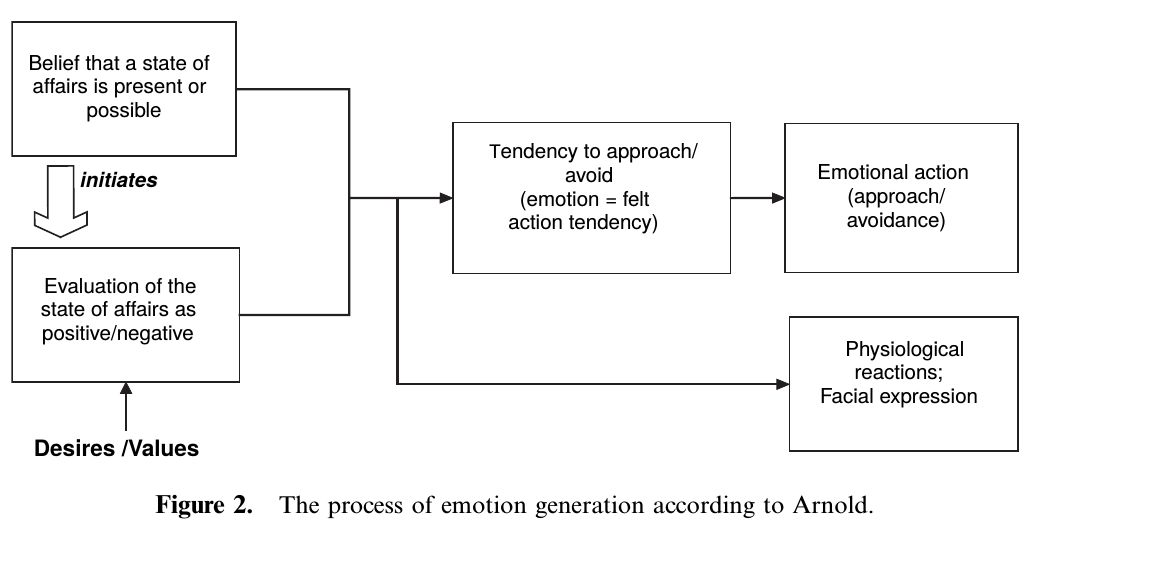
\includegraphics[width=0.8\textwidth]{arnold.jpg}
 \caption{\label{fig:procedure} Emotiontheorie arnold.}
\end{figure}

In 1962 veröffentlichte Sylvan Tomkins sein Buch "Affect, Imagery, Consciousness", womit er als Begründer der Basisemotionstheorie gilt. Tomkins beschreibt dabei 9 universelle Emotionen, wobei sechs von ihnen in zwei verschiedenen Steigerungsformen auftreten. Diese sechs Emotionen sind Interesse/ Begeisterung, Vergnügen/ Freude, Überraschung/ Erschrecken, Leid/Qual, Ärger/Wut und Angst/ Grauen. Die letzten sind Scham/ Demütigung und Ekel vor schlechten Geruch/Geschmack. Wie grundlegend in allen Basisemotionstheorien die folgten, hält er diese Emotionen für elementar und universell. Es wird angenommen, dass sie evolutionär geprägt und vererbt werden. Dabei werden diese Emotionen automatisch von Objekten oder 
Ereignissen ausgelöst. Dabei sind die Emotionen sowohl biologisch analog, wobei dies meint dass  alle Emotionen mit dem gleichen Name dieselben Muster im Verhalten, Körperreaktion und Gesichtsausdruck und Erfahrungen verbunden sind. Durch diese gleichen Muster können Menschen in der ganzen Welt einfach und effektive diese Basisemotionen erkennen und verstehen.Sie sind außerdem homogen, weil sie von derselben Ursache ausgelöst werden.\\

Im selben Jahr publizierten Schachter und Singer ihre Emotionstheorie, die auf verschiedene Weise interpretiert wurde. Zum einen als Zwei-Faktoren-Theorie. Wobei eine Emotion maßgeblich von der kognitiven Interpretation einer Situation und dem Arousal abhängt. Durch diesen Zusammenhang mit dem Arousal als körperliche Reaktion wird die Theorie als Neo-Jamesische Theorie bezeichnet und zum anderen aufgrund ihren kognitiven Anteils zu der Appraisal-Theorien. Ein Emotionserlebnis hängt laut Schachter und Singer von drei Faktoren ab:

\begin{enumerate}
\item eine Situation muss emotionsauslösend interpretiert werden
\item es erfolgt eine unspezifische, physiologische Aktivierung
\item dabei muss die emotionale Situation als Ursache für die unspezifische, physiologische Aktivierung interpretiert werden
\end{enumerate}

Die Höhe der physiologischen Aktivierung beeinflusst dabei die Intensität der Emotion. Die Interpretation der Situation beeinflusst dabei die Qualität der Emotion. Allerdings konnten die Experiment und deren Ergebnisse durch Reisenzein nicht oder nur teilweise reproduziert werden. Im Detail wurden folgende Zusammenhänge überprüft:
\begin{itemize}
\item Dämpfung der physiologischen Erregung führt zur Dämpfung des Emotionserlebnisses - konnte nicht nachgewiesen werden

\item Reinterpretation eines Teils der aktuellen Erregung auf eine "neutrale" Ursache führt zu einer Verminderung des Emotionserlebnisses - konnte nicht nachgewiesen werden

\item Erregungsreste aus Situation A führen nach Beendigung bei nachfolgender Situation B zu einer Verstärkung des Gefühlserlebnisses - nachgewiesen Zillmanscher Erregungstransfer
\end{itemize}

Valin konnte sogar nachweisen, dass eine eingebildete Erregung eine emotionale Reaktion hervorrufen konnte. \\










%Mit diesen zwei Richtungen Appraisal- und Basisemotionstheorien wurden bis 2009 alle Theorien eingeordnet. allerdings gibt es laut Gendron und Barett, welche die historische Einordnung der Emotionstheorien neu rekonstruierten und dabei eine weitere Strömung die psychologisch konstruktivistischen Emotionstheorien definierten.
%Basierend auf der Zwei-Faktoren-Theorie von Schachter und Singer, welche laut ihnen einen Apraisal- Basisemotionen Dualismus aufweist, haben sie unter Einbeziehung vernachlässigter Emotionsarbeiten aus den Dunkelalter der Emotionen den Psychologischen Konstruktivismus konstruiert.





%Im Kern sagt Tomkins’ Affekttheorie, dass alle Menschen exakt neun unterschiedliche Affekte besitzen, die genetisch programmiert und nicht kulturell erworben sind. Die am frühesten entwickelten sechs davon werden von Tomkins als zweistufig beschrieben, wobei die zweite Stufe eine Steigerung der ersten Stufe darstellt: Interesse/Begeisterung, Vergnügen/Freude, Überraschung/Erschrecken, Leid/Qual, Ärger/Wut und Angst/Grauen. Ein weiteres Paar ist entwicklungsgeschichtlich jünger: Scham/Demütigung. Die letzten zwei sind Ekel vor schlechtem Geruch (Tomkins erfand dafür das Wort dismell) und Ekel vor schlechtem Geschmack. Tomkins sieht diese neun Affekte als diskret und elementar an, im Gegensatz zu Emotionen, die komplex und zusammengesetzt sind. Die Affekte des Menschen sind s.E. verwandt mit denen höherer Tiere und nicht zu verwechseln mit den Trieben nach Sigmund Freud. (Siehe auch Abschnitt Affekttheorie im Hauptartikel Psychoanalyse)

%Nach Tomkins und seinem Schüler Paul Ekman gibt es charakteristische und global universelle Gesichtsausdrücke für die Affekte.[7] Die Tatsache, dass selbst blind geborene Kinder diese charakteristischen Gesichtsausdrücke zeigen, wird als Beweis für die angeborene Natur der Affekte angeführt.


%Zur Anfangszeit der institutionalisierten Psychologie (im letzten Drittel des 19. Jahrhunderts) hat man sich zwar recht intensiv mit den Emotionen befasst. Die Psychologie verstand sich damals als Wissenschaft von den Bewusstseinszuständen und Emotionen manifestieren sich zweifellos (zumindest unter anderem) im Erleben. Nach dem Aufkommen des Behaviorismus (um 1915) und der damit verbundenen, vorübergehenden Neudefinition der Psychologie als »Wissenschaft vom Verhalten« wurden die Emotionen allerdings zunehmend vernachlässigt. Im Jahre 1933 sagte der amerikanische Behaviorist Max F. Meyer sogar vorher, die wissenschaftliche Psychologie würde die Beschäftigung mit Emotionen spätestens 1950 als eine Kuriosität vergangener Zeiten belächeln (Meyer, 1933). Statt dessen erlebte die wissenschaftliche Psychologie in den 1950er Jahren jedoch den Niedergang des Behaviorismus. Aber auch die dem Behaviorismus nachfolgende, am Modell der Informationsverarbeitung in Computern orientierte Kognitive Psychologie hat die Emotionen zunächst vernachlässigt. Zum Teil glaubte man, wie schon vorher Meyer (1933), die Kategorie »Emotion« würde sich in nichtemotionale Kategorien auflösen lassen, wie zum Beispiel die Kategorien »körperliche Aktivierung« und »Kognition« (Mandler, 1984; Schachter, 1964). Es spricht jedoch vieles dafür, dass eine Reduktion von Emotionen auf nichtemotionale Zustände nicht möglich ist. Ein zweiter Grund für die Renaissance der Emotionsforschung ist, dass es in den letzten 30 Jahren zu einer Neubewertung der Adaptivität von Emotionen gekommen ist. Traditionell herrschte in der Psychologie und auch in anderen Humanwissenschaften die Ansicht vor, die Emotionen seien Überbleibsel der evolutionären Vergangenheit des Menschen, die zumindest in der modernen Gesellschaft wenig Nutzen hätten (vgl. Arnold, 1960). Was den Menschen nach dieser Sicht auszeichnet, ist sein Verstand, seine Fähigkeit zum vernünftigen Denken und Entscheiden. Dabei seien die Emotionen – als angebliche Produkte primitiver, in archaischen Hirnregionen beheimateter Affektprogramme – nur störend: Sie beeinträchtigen das vernünftige Denken und führen als Folge davon zu Handlungen, die den eigenen besten Interessen der Person zuwiderlaufen. Aus dieser Perspektive gesehen mag die Erforschung der Emotionen nur zu dem Grad wichtig erscheinen, als sie uns in die Lage versetzt, unsere Emotionen besser in den Griff zu bekommen (vgl. Gross, 2008). In den letzten dreißig Jahren hat sich dagegen zunehmend die – historisch freilich nicht wirklich neue (z.B. McDougall, 1908/1960; Meinong, 1894) – Auffassung durchgesetzt, dass Emotionen, auch wenn sie ohne Zweifel manchmal schädliche Effekte haben, insgesamt adaptiv sind (Feldman Barrett u. Salovey, 2002; Frijda, 1994; s. dazu auch Reisenzein u. Horstmann, 2006). Nach Ansicht einiger Forscher sind Emotionen sogar unverzichtbar für adaptives Handeln (z.B. Damasio, 1994). Zumindest aber wird heute in der Psychologie und zunehmend auch in anderen Humanwissenschaften die alltagspsychologische Erkenntnis akzeptiert, dass Emotionen in der »psychischen Maschinerie« eine wichtige Rolle spielen und dass man deshalb ohne die Berücksichtigung der Emotionen nicht ausreichend verstehen kann, wie Menschen »funktionieren«, das heißt, weshalb sie so denken und handeln, wie sie es tun.
V
